\documentclass[convert]{standalone}

\usepackage{tikz}
\pagestyle{empty}

% INT_AY22_L03_Fig10_Tangent-line.png

\begin{document}
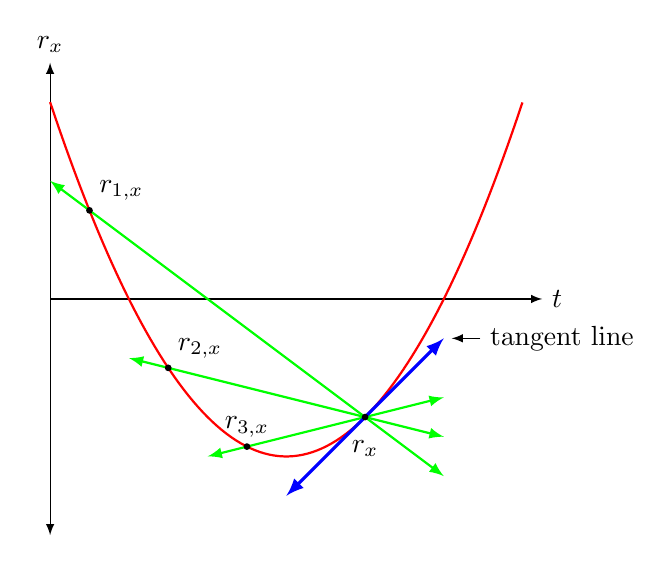
\begin{tikzpicture}[> = latex]

	% Graph axes
	
	\draw [<->] (0, -3) -- (0, 3) node [above] {$r_x$};
	\draw [->] (0, 0) -- (6.25, 0) node [right] {$t$};
	
	% Graph curve
	
	\draw [red, thick] plot [variable = \t, domain = 0 : 6, samples = 100] ({\t}, {0.5 * (\t - 3)^2 - 2});
	
	% Secant line limiting process
	
	\begin{scope}[thick, green, <->]
	
		\draw (0, 1.5) -- (5, -2.25);
		\draw (1, -0.75) -- (5, -1.75);
		\draw (2, -2) -- (5, -1.25);
	
	\end{scope}
	
	\draw [fill = black] (0.5, 1.125) circle (1 pt) node [above right] {$r_{1, x}$};
	\draw [fill = black] (1.5, -0.875) circle (1 pt) node [above right] {$r_{2, x}$};
	\draw [fill = black] (2.5, -1.875) circle (1 pt) node [above] {$r_{3, x}$};
	
	% Tangent line
	
	\draw [very thick, blue, <->] (3, -2.5) -- (5, -0.5);
	\draw [fill = black] (4, -1.5) circle (1 pt) node [below = 0.5 em] {$r_x$};
	
	\node (secant) at (6.5, -0.5) {tangent line};
	\draw [->] (secant.west) -- (5.1, -0.5);
	
\end{tikzpicture}
\end{document}